\section{Prior Work and Project Proposal} \label{sec:prior}

We build our project on the prior work done on LSSD~\cite{nowatzki2016pushing} (Work done in Vertical Research Group), which includes identification of specialization principles and proposal of the
high-level architecture of the high throughput compute engine (called Softbrain now). Softbrain builds 
upon the LSSD principles and implements the general micro-architectural mechanisms identified in prior work. 
Before explaining the high level organization of Proximate architecture, the five
specialization principles employed to consider this style of accelerator architecture are explained. 
The primary insight 
on coming to the architectural substrate is based on well-understood mechanisms of specialization used in
DSAs. 

\subsection{Specialization Principles}
Broadly, these principles are seen in as a counterpart to the insights from Hameed et al.~\cite{1815968}, in that they describe the sources of inefficiency in a general purpose processor, whereas our findings are oriented around
elucidating the sources of potential efficiency gain from specialization.

\paragraph{Concurrency Specialization}
The concurrency of a workload is the degree to which its operations can be
performed in parallel. This concurrency can be derived from data or thread level parallelism found in the
workloads. Examples of specialization strategies include employing many independent processing elements
with their own controllers, or using a wide vector model with a single controller. The former one is chosen as
baseline architecture having many processing elements with a low-power controller.

\paragraph{Computation Specialization} Computations are individual units of work in an algorithm executed by
functional units (FUs). Specializing computation means creating problem-specific FUs. For instance, a sin
FU would much more efficiently compute the sine function than iterative methods on a general purpose
processor. Specializing computation improves performance and energy by reducing the total work. Most of
the neural network applications employ some commonality in FU types.

\paragraph{Communication Specialization} Communication is the means of transmission of transient values between
the storage and functional units. Specialized communication is simply the instantiation of communication
channels, and potentially buffering, between FUs to ultimately facilitate a faster operand throughput to the
FUs. This reduces power by lessening access to intermediate storage, and potentially area if the alternative is
a general communication network.

\paragraph{Data Reuse Specialization} Data reuse is an algorithmic property where intermediate computed values
are consumed multiple times. The specialization of data reuse means using custom storage structures or
reuse buffers for these temporaries. Specializing reuse benefits performance and power by avoiding the more
expensive access to a larger global memory or register files.

\paragraph{Coordination Specialization} Hardware coordination is the management of multiple hardware units and
their timing to perform work. Instruction sequencing, control flow, interrupts handling and address generation
are all examples of coordination tasks. Specializing it usually involves the creation of small finite state
machines to perform each task. A low-power in-order core or a micro-controller could be used for this
coordination specialization. Based on the this principle, to aim at high concurrency workloads and provide 
the task/data locality to 
programmers, Proximate has lot of  such small in-order cores acting both 
as coordination unit and computation engine to execute irregular workloads. This is based heavily on the 
principle of having many small in-order cores near memory to do the high-throughput computation~\cite{menon2014memory}.

Based on extensions to all the prior work explained above,
we currently have built a vector dataflow programmable accelerator 
called Softbrain that is general purpose  
programmable using a high level hardware 
programming interface (HPI). 
Regular streaming workloads that are mainly 
single threaded showed comparable performance to the 
fixed function implementation of these workloads. 
The current research also aims at having a general purpose 
programmable tiled organization of 
in-order cores which run single threaded fine-grained parallel tasks,
connected to the programmable accelerator (Softbrain) briefed above. 
Together this entire hardware organization targets both 
irregular and regular workloads, and we call 
this combined organization of hardware as Proximate. 
Proximate combines this multi-core tiled architecture with
programmable/specialized accelerator (Softbrain) together into a 
single external PCIE device. Figure~\ref{fig:prx-orig} shows high-level
overview of the current Proximate offload engine. 

\begin{figure}
  \begin{center}
    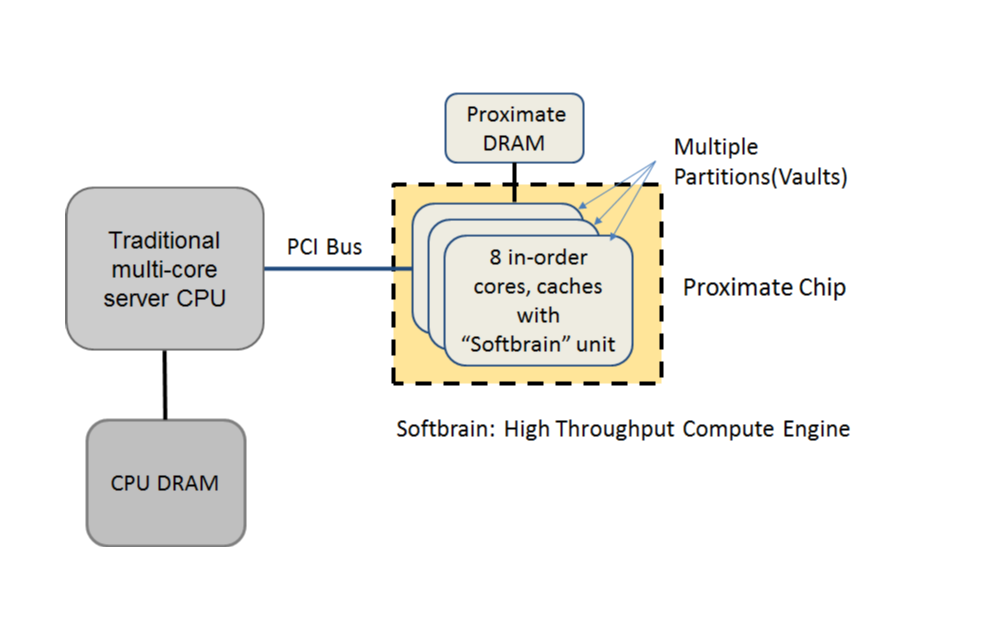
\includegraphics[width=\linewidth]{cs758-figs/prx-orig.png}
  \end{center}
\vspace{-0.9in}
  \caption{Proximate Offload Engine}
  \label{fig:prx-orig}
\vspace{-0.05in}
\end{figure}

Proximate has a 16 compute tiles, 
each compute tile with 8 (RISC-V) in-order cores, 
a programmable/specialized accelerator (softbrain
fabric) for a total of 128 RISC-V inorder cores and 
16 softbrain fabric instances connected to a common 
memory hierarchy. It is programmable using a high-level 
offload API to offload the data, allocate memory on device and 
copy the data to/from the host processor. 


\subsection{Project Proposed}
Since, we exactly cannot have the same hardware model setting as Figure~\ref{fig:prx-orig},
for our project, we have to slightly modify the API as well as the hardware model to suit our experiments.
Figure~\ref{fig:prx} shows the organization of the entire device for our
project purposes. We assume both the host core and the proximate device
to be located in the same shared address space and proximate operates
in a memory mapped region of the shared address space. 
The host core also runs the Proximate parallel programming API and the runtime
is responsible for offloading the tasks at coarser-granularity to a device-specific
task scheduler. This task scheduler is connected to the proximate tiles, with each tile
having group of in-order cores and the high-throughput compute engine, Softbrain. 


\begin{figure*}[h]
  \begin{center}
    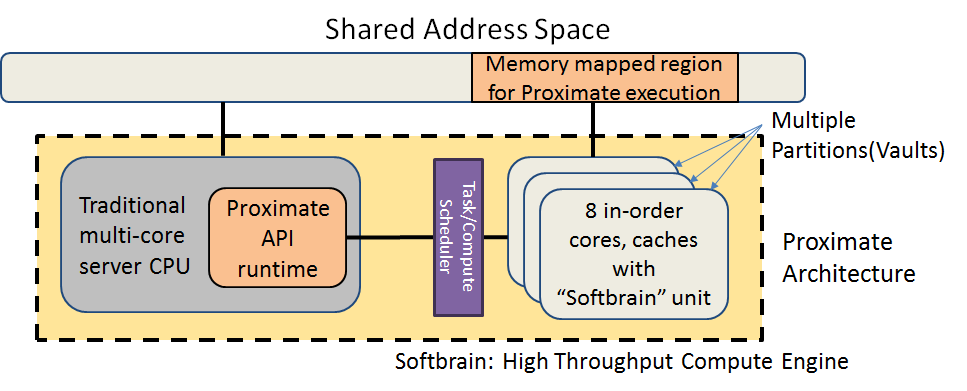
\includegraphics[width=\linewidth]{cs758-figs/proj.png}
  \end{center}
\vspace{-0.2in}
  \caption{Proximate Architecture in Our Project Setting}
  \label{fig:prx}
\vspace{-0.05in}
\end{figure*}

This project aims to parallelize some of the 
single-threaded regular HPC workloads and 
irregular workloads on Proximate architecture 
and evaluate performance and bandwidth 
limitations compared to a server class chip 
like 64-core Xeon Phi Knights landing.
We start this by converting all the single-threaded workloads
to the parallel versions of pthreads and OpenMP. Th idea behind this
is to get the data from real hardware as well as see the scalability of these parallel workloads.
We then implement the proximate versions of the parallel programs and evaluate the performance
w.r.t to the best configuration of pthread run on Xeon-Phi. 



